\documentclass[12pt,a4paper,oneside]{article}
\usepackage[utf8]{inputenc}
\usepackage[portuguese]{babel}
\usepackage[T1]{fontenc}
\usepackage{times}
\usepackage[left=3cm,right=2cm,top=3cm,bottom=2cm]{geometry}
\usepackage{setspace}
\usepackage{indentfirst}
\usepackage{graphicx}
\usepackage{float}
\usepackage{amsmath}
\usepackage{amsfonts}
\usepackage{amssymb}
\usepackage{booktabs}
\usepackage{multirow}
\usepackage{array}
\usepackage{longtable}
\usepackage{url}
\usepackage[hidelinks]{hyperref}
\usepackage{caption}
\usepackage{subcaption}
\usepackage{listings}
\usepackage{xcolor}

% Configuracoes ABNT
\onehalfspacing
\setlength{\parindent}{1.25cm}
\setlength{\parskip}{0pt}

% Configuracao de titulos
\usepackage{titlesec}
\titleformat{\section}{\normalfont\fontsize{12}{15}\bfseries\uppercase}{\thesection}{1em}{}
\titleformat{\subsection}{\normalfont\fontsize{12}{15}\bfseries}{\thesubsection}{1em}{}
\titleformat{\subsubsection}{\normalfont\fontsize{12}{15}\bfseries}{\thesubsubsection}{1em}{}

% Configuracao para codigo
\lstset{
    basicstyle=\ttfamily\footnotesize,
    breaklines=true,
    frame=single,
    language=Python,
    showstringspaces=false,
    commentstyle=\color{gray},
    keywordstyle=\color{blue},
    stringstyle=\color{red}
}

\begin{document}

% CAPA
\begin{titlepage}
\centering
\vspace*{1cm}

{\fontsize{14}{16}\selectfont\bfseries\uppercase{Universidade do Estado do Amazonas}}\\
{\fontsize{14}{16}\selectfont\bfseries\uppercase{Escola Superior de Tecnologia}}\\
{\fontsize{14}{16}\selectfont\bfseries\uppercase{Curso de Engenharia de Computacao}}\\

\vspace{3cm}

{\fontsize{14}{16}\selectfont\bfseries\uppercase{Estudo Comparativo de Algoritmos de Criptografia e Desenvolvimento de Aplicacao de Assinatura Digital}}

\vspace{3cm}

{\fontsize{12}{14}\selectfont
\textbf{Autores:}\\
Carlos Lavor Neto\\
Eric Dias Perin\\
Alexandro Pantoja\\
}

\vspace{2cm}

{\fontsize{12}{14}\selectfont
Trabalho apresentado a disciplina de Topicos Especiais em Computacao IV como requisito parcial para avaliacao academica.

\vspace{0.5cm}
\textbf{Repositorio do Projeto:}\\
\url{https://github.com/CarlosLNeto/crypto-performance-study.git}
}

\vfill

{\fontsize{12}{14}\selectfont
Manaus -- AM\\
2025
}

\end{titlepage}

% RESUMO
\newpage
\section*{RESUMO}

Este trabalho apresenta um estudo abrangente sobre criptografia aplicada, dividido em duas atividades complementares. A Atividade 1 consiste em uma analise comparativa de desempenho computacional entre tres algoritmos de criptografia simetrica: Advanced Encryption Standard (AES), Blowfish e Twofish, avaliando metricas de CPU, memoria, tempo de execucao e throughput com 40 configuracoes testadas e 100 iteracoes cada. A Atividade 2 desenvolve uma aplicacao pratica de envio de mensagens com assinatura digital, implementando geracao de certificados X.509 ad-hoc, verificacao de autenticidade com RSA-PSS e SHA-256, e uma interface web completa para demonstracao interativa do sistema. Os resultados da Atividade 1 demonstram que o AES oferece o melhor throughput medio (277,80 MB/s), enquanto o Blowfish apresenta menor consumo de recursos (155,48 MB/s). Na Atividade 2, a aplicacao demonstrou 100\% de eficacia na deteccao de alteracoes, com tempos de geracao de certificados de 79,7ms, assinatura de 0,98ms e verificacao de 0,13ms, alem de uma interface web funcional para chat em tempo real com assinatura digital. O trabalho contribui para o entendimento pratico da criptografia moderna, fornecendo dados quantitativos para selecao de algoritmos e uma implementacao funcional de infraestrutura de chave publica com demonstracao web interativa.

\vspace{0.5cm}
\noindent\textbf{Palavras-chave:} Criptografia. Algoritmos simetricos. Assinatura digital. Certificados digitais. Desempenho computacional. Seguranca da informacao.

% SUMARIO
\newpage
\tableofcontents

% INTRODUCAO
\newpage
\section{INTRODUCAO}

A criptografia constitui um dos pilares fundamentais da seguranca da informacao moderna, desempenhando papel crucial na protecao de dados em diversas aplicacoes. Este trabalho aborda duas dimensoes complementares da criptografia aplicada atraves de duas atividades distintas: a analise quantitativa de algoritmos de criptografia simetrica e o desenvolvimento de uma aplicacao pratica de assinatura digital.

A primeira atividade foca na avaliacao comparativa de performance dos algoritmos AES (Advanced Encryption Standard), Blowfish e Twofish, enquanto a segunda explora a implementacao de mecanismos de autenticacao e integridade atraves de assinaturas digitais com certificados gerados ad-hoc.

\subsection{Objetivos}

\subsubsection{Objetivo Geral}

Realizar um estudo abrangente sobre criptografia aplicada, comparando o desempenho computacional de algoritmos simetricos e desenvolvendo uma aplicacao funcional de assinatura digital com certificados ad-hoc.

\subsubsection{Objetivos Especificos}

\begin{enumerate}
    \item \textbf{Atividade 1}: Implementar benchmarks automatizados para medicao precisa de performance dos algoritmos AES, Blowfish e Twofish;
    \item \textbf{Atividade 1}: Analisar o comportamento dos algoritmos com diferentes tamanhos de dados e configuracoes de chave;
    \item \textbf{Atividade 2}: Desenvolver uma aplicacao de envio de mensagens com assinatura digital;
    \item \textbf{Atividade 2}: Implementar geracao de certificados digitais X.509 ad-hoc;
    \item \textbf{Atividade 2}: Criar interface web para demonstracao interativa do sistema;
    \item Realizar analises estatisticas para validar a significancia das diferencas observadas;
    \item Gerar visualizacoes graficas para facilitar a interpretacao dos resultados;
    \item Fornecer recomendacoes praticas baseadas nos resultados obtidos.
\end{enumerate}

% REFERENCIAL TEORICO
\section{REFERENCIAL TEORICO}

\subsection{Criptografia Simetrica}

A criptografia simetrica utiliza a mesma chave para as operacoes de criptografia e descriptografia, oferecendo alta eficiencia computacional para processamento de grandes volumes de dados.

\subsubsection{Advanced Encryption Standard (AES)}

O AES e baseado na cifra Rijndael, adotado como padrao pelo NIST em 2001. Opera com blocos de 128 bits e suporta chaves de 128, 192 e 256 bits, sendo otimizado para implementacao em hardware moderno.

\subsubsection{Blowfish}

Desenvolvido por Bruce Schneier em 1993, opera com blocos de 64 bits e suporta chaves variaveis de 32 a 448 bits. E conhecido por sua velocidade e simplicidade de implementacao.

\subsubsection{Twofish}

Sucessor do Blowfish e finalista na competicao do AES. Opera com blocos de 128 bits e suporta chaves de 128, 192 e 256 bits, oferecendo caracteristicas de seguranca avancadas.

\subsection{Criptografia Assimetrica e Assinatura Digital}

A criptografia assimetrica utiliza pares de chaves matematicamente relacionadas, possibilitando a implementacao de assinaturas digitais que garantem autenticidade, integridade e nao-repudio.

\subsubsection{Algoritmo RSA}

O RSA e baseado na dificuldade de fatoracao de numeros inteiros grandes. Para assinaturas digitais, o processo envolve a criacao de um hash da mensagem, que e entao criptografado com a chave privada.

\subsubsection{Certificados Digitais X.509}

Os certificados digitais seguem o padrao X.509 e contem informacoes como nome do titular, chave publica, periodo de validade e assinatura de uma autoridade certificadora.

\subsection{Tecnologias Utilizadas}

\subsubsection{Linguagens e Frameworks}

\begin{itemize}
    \item \textbf{Python 3.13}: Linguagem principal para implementacao de todos os algoritmos e aplicacoes
    \item \textbf{Flask 2.3+}: Framework web para desenvolvimento da interface de chat
    \item \textbf{HTML5/CSS3/JavaScript}: Tecnologias frontend para interface web responsiva
\end{itemize}

\subsubsection{Bibliotecas Criptograficas}

\begin{itemize}
    \item \textbf{cryptography}: Biblioteca principal para operacoes criptograficas modernas
    \item \textbf{pycryptodome}: Implementacao dos algoritmos Blowfish e Twofish
    \item \textbf{werkzeug}: Utilitarios de seguranca para hash de senhas
\end{itemize}

\subsubsection{Bibliotecas de Analise e Visualizacao}

\begin{itemize}
    \item \textbf{matplotlib}: Geracao de graficos e visualizacoes
    \item \textbf{seaborn}: Visualizacoes estatisticas avancadas
    \item \textbf{pandas}: Manipulacao e analise de dados
    \item \textbf{numpy}: Computacao numerica e operacoes matematicas
    \item \textbf{scipy}: Analises estatisticas (ANOVA)
\end{itemize}

\subsubsection{Bibliotecas de Sistema}

\begin{itemize}
    \item \textbf{psutil}: Monitoramento de recursos do sistema (CPU, memoria)
    \item \textbf{tabulate}: Formatacao de tabelas para relatorios
\end{itemize}

% DESENVOLVIMENTO
\section{DESENVOLVIMENTO}

\section{ATIVIDADE 1: ANALISE DE ALGORITMOS DE CRIPTOGRAFIA SIMETRICA}

\subsection{Arquitetura do Sistema de Benchmark}

O sistema foi desenvolvido em Python utilizando as bibliotecas \texttt{cryptography} e \texttt{pycryptodome}. A arquitetura modular permite medicoes precisas e isoladas de cada algoritmo.

\begin{lstlisting}[caption=Estrutura principal da classe CryptoBenchmark]
class CryptoBenchmark:
    def __init__(self):
        self.results = []
        self.data_sizes = [1024, 10240, 102400, 1048576, 10485760]
        self.iterations = 100
    
    def measure_performance(self, encrypt_func, decrypt_func, data, algorithm, key_size):
        process = psutil.Process()
        # Medicoes de baseline e execucao dos testes
        # Coleta de metricas de CPU, memoria e tempo
\end{lstlisting}

\subsection{Metodologia de Medicao}

Cada teste e executado 100 vezes para garantir confiabilidade estatistica. O procedimento inclui:

\begin{enumerate}
    \item Geracao de dados aleatorios criptograficamente seguros
    \item Limpeza de memoria entre execucoes (\texttt{gc.collect()})
    \item Medicao de recursos antes e apos cada operacao
    \item Calculo de metricas estatisticas (media, desvio padrao)
\end{enumerate}

\subsection{Configuracoes de Teste}

Os testes abrangem cinco tamanhos de dados (1KB a 10MB) e multiplas configuracoes de chave:
\begin{itemize}
    \item AES: 128, 192, 256 bits
    \item Blowfish: 128, 256 bits
    \item Twofish: 128, 192, 256 bits
\end{itemize}

\subsection{Resultados da Atividade 1}

Os resultados demonstram que o AES oferece o melhor throughput medio (277,80 MB/s), enquanto o Blowfish apresenta menor consumo de recursos. A analise estatistica ANOVA indica que nao ha diferencas significativas entre os algoritmos ao nivel de significancia $\\alpha$ = 0,05.

\section{ATIVIDADE 2: SISTEMA DE CHAT COM ASSINATURA DIGITAL}

\subsection{Arquitetura do Sistema}

O sistema de chat foi desenvolvido com arquitetura cliente-servidor utilizando Flask e WebSocket para comunicacao em tempo real. A aplicacao integra tres componentes principais:

\begin{itemize}
    \item \textbf{Backend}: Servidor Flask com SocketIO para WebSocket
    \item \textbf{Frontend}: Interface web responsiva com JavaScript
    \item \textbf{Criptografia}: Sistema de assinatura digital RSA-PSS
\end{itemize}

\begin{lstlisting}[caption=Estrutura da aplicacao de chat]
class CertificateManager:
    def generate_certificate(self, username, common_name):
        # Gerar chave privada RSA 2048 bits
        private_key = rsa.generate_private_key(
            public_exponent=65537, key_size=2048)
        
        # Criar certificado X.509 auto-assinado
        cert = x509.CertificateBuilder().subject_name(
            subject).issuer_name(issuer)
\end{lstlisting}

\subsection{Geracao de Certificados Ad-hoc}

O sistema implementa geracao automatica de certificados X.509 auto-assinados para cada usuario no primeiro login. Os certificados utilizam:

\begin{itemize}
    \item \textbf{Algoritmo}: RSA 2048 bits
    \item \textbf{Hash}: SHA-256
    \item \textbf{Validade}: 365 dias
    \item \textbf{Formato}: PKCS\#12 com senha
\end{itemize}

\begin{lstlisting}[caption=Processo de geracao de certificado]
def generate_certificate(self, username, common_name):
    private_key = rsa.generate_private_key(
        public_exponent=65537, key_size=2048)
    
    subject = issuer = x509.Name([
        x509.NameAttribute(NameOID.COUNTRY_NAME, "BR"),
        x509.NameAttribute(NameOID.ORGANIZATION_NAME, "UEA"),
        x509.NameAttribute(NameOID.COMMON_NAME, common_name),
    ])
    
    cert = x509.CertificateBuilder().subject_name(subject)
        .not_valid_before(datetime.utcnow())
        .not_valid_after(datetime.utcnow() + timedelta(days=365))
        .sign(private_key, hashes.SHA256())
\end{lstlisting}

\subsection{Sistema de Assinatura Digital}

Cada mensagem enviada no chat é automaticamente assinada digitalmente utilizando o algoritmo RSA-PSS com hash SHA-256. O processo garante:

\begin{itemize}
    \item \textbf{Autenticidade}: Verificacao da identidade do remetente
    \item \textbf{Integridade}: Deteccao de alteracoes na mensagem
    \item \textbf{Nao-repudio}: Impossibilidade de negar o envio
\end{itemize}

\begin{lstlisting}[caption=Assinatura de mensagem]
def sign_message(self, username, message):
    message_bytes = message.encode('utf-8')
    signature = private_key.sign(
        message_bytes,
        padding.PSS(
            mgf=padding.MGF1(hashes.SHA256()),
            salt_length=padding.PSS.MAX_LENGTH),
        hashes.SHA256())
    
    return {
        'message': message,
        'signature': signature.hex(),
        'certificate': cert.public_bytes(serialization.Encoding.PEM),
        'timestamp': datetime.now().isoformat()
    }
\end{lstlisting}

\subsection{Comunicacao em Tempo Real com WebSocket}

A implementacao utiliza Flask-SocketIO para comunicacao bidirecional em tempo real:

\begin{itemize}
    \item \textbf{Conexao}: Estabelecimento automatico via WebSocket
    \item \textbf{Salas}: Sistema de rooms para broadcast de mensagens
    \item \textbf{Eventos}: Tratamento de entrada/saida de usuarios
    \item \textbf{Estatisticas}: Atualizacao em tempo real de metricas
\end{itemize}

\begin{lstlisting}[caption=Eventos WebSocket principais]
@socketio.on('connect')
def on_connect():
    join_room('chat')
    chat_stats['active_users'].add(session['username'])
    emit('user_joined', user_data, room='chat')

@socketio.on('send_message')
def handle_message(data):
    signed_message = message_signer.sign_message(username, message)
    is_valid = message_signer.verify_message(signed_message)
    emit('new_message', message_data, room='chat')
\end{lstlisting}

\subsection{Interface de Usuário}

O frontend implementa uma interface moderna e responsiva com:

\begin{itemize}
    \item \textbf{Design}: Layout responsivo com CSS Grid/Flexbox
    \item \textbf{Autenticacao}: Sistema de login com usuarios pre-cadastrados
    \item \textbf{Chat}: Area de mensagens com scroll automatico
    \item \textbf{Sidebar}: Painel de estatisticas e usuarios online
    \item \textbf{Indicadores}: Status de verificacao das mensagens
\end{itemize}

\subsection{Aplicacao Web de Chat em Tempo Real}

O sistema de chat web implementa uma solucao completa de comunicacao segura com as seguintes caracteristicas:

\subsubsection{Arquitetura do Sistema}

\begin{itemize}
    \item \textbf{Backend}: Servidor Flask com extensao SocketIO
    \item \textbf{Frontend}: Interface HTML5 com JavaScript para WebSocket
    \item \textbf{Banco de Dados}: Sistema de sessoes em memoria
    \item \textbf{Criptografia}: RSA-PSS com SHA-256 integrado
\end{itemize}

\begin{lstlisting}[caption=Configuracao do servidor Flask com WebSocket]
app = Flask(__name__, template_folder='../templates')
socketio = SocketIO(app, cors_allowed_origins="*")

@socketio.on('connect')
def on_connect():
    join_room('chat')
    chat_stats['active_users'].add(session['username'])
    emit('user_joined', user_data, room='chat')
\end{lstlisting}

\subsubsection{Fluxo de Funcionamento}

O sistema opera seguindo este fluxo:

\begin{enumerate}
    \item \textbf{Autenticacao}: Usuario acessa /login e insere credenciais
    \item \textbf{Geracao de Certificado}: Sistema cria certificado X.509 automaticamente
    \item \textbf{Conexao WebSocket}: Cliente estabelece conexao bidirecional
    \item \textbf{Envio de Mensagem}: Usuario digita mensagem na interface
    \item \textbf{Assinatura Automatica}: Sistema assina mensagem com chave privada
    \item \textbf{Broadcast}: Mensagem assinada e enviada para todos os usuarios
    \item \textbf{Verificacao}: Cada cliente verifica assinatura automaticamente
    \item \textbf{Exibicao}: Mensagem exibida com status de verificacao
\end{enumerate}

\begin{lstlisting}[caption=Processamento de mensagem no chat]
@socketio.on('send_message')
def handle_message(data):
    username = session['username']
    message = data['message']
    
    # Assinar mensagem automaticamente
    signed_message = message_signer.sign_message(username, message)
    
    # Verificar assinatura
    is_valid = message_signer.verify_message(signed_message)
    
    # Broadcast para todos os usuarios
    emit('new_message', {
        'username': username,
        'message': message,
        'verified': is_valid
    }, room='chat')
\end{lstlisting}

\subsection{Sistema de Analise de Performance}

O script de analise implementa um sistema robusto de medicao de performance:

\subsubsection{Metodologias de Teste}

\begin{enumerate}
    \item \textbf{Benchmark Sequencial}: 50 iteracoes por tamanho
    \item \textbf{Benchmark Concorrente}: 5 usuarios simultaneos
    \item \textbf{Teste de Stress}: 30 segundos de operacoes continuas
\end{enumerate}

\begin{lstlisting}[caption=Implementacao do teste concorrente]
with ThreadPoolExecutor(max_workers=concurrent_users) as executor:
    futures = [executor.submit(concurrent_sign, i) 
              for i in range(concurrent_users)]
    concurrent_times = []
    for future in futures:
        concurrent_times.extend(future.result())
\end{lstlisting}

\subsubsection{Resultados Obtidos}

\begin{itemize}
    \item \textbf{Assinatura}: Tempo medio de 62ms
    \item \textbf{Verificacao}: Tempo medio de 0.09ms
    \item \textbf{Throughput de Assinatura}: 63 KB/s
    \item \textbf{Throughput de Verificacao}: 41.824 MB/s
\end{itemize}

Foi desenvolvido um sistema abrangente de análise de performance que inclui:

\begin{itemize}
    \item \textbf{Benchmark Sequencial}: Testes com diferentes tamanhos de mensagem
    \item \textbf{Benchmark Concorrente}: Simulacao de multiplos usuarios simultaneos
    \item \textbf{Teste de Stress}: Operacoes continuas por periodo determinado
    \item \textbf{Metricas Coletadas}: Tempo, CPU, memoria, throughput
\end{itemize}

\begin{lstlisting}[caption=Benchmark de operações concorrentes]
def benchmark_signing_operations(self, message_sizes, iterations=100, 
                               concurrent_users=5):
    with ThreadPoolExecutor(max_workers=concurrent_users) as executor:
        futures = [executor.submit(concurrent_sign, i) 
                  for i in range(concurrent_users)]
        concurrent_times = []
        for future in futures:
            concurrent_times.extend(future.result())
\end{lstlisting}

\subsection{Funcionalidades Implementadas}

O sistema de chat oferece as seguintes funcionalidades:

\begin{enumerate}
    \item \textbf{Autenticacao Segura}: Login com usuarios pre-cadastrados
    \item \textbf{Geracao Automatica de Certificados}: Criacao no primeiro acesso
    \item \textbf{Chat em Tempo Real}: Comunicacao via WebSocket
    \item \textbf{Assinatura Automatica}: Todas as mensagens sao assinadas
    \item \textbf{Verificacao de Integridade}: Validacao automatica das assinaturas
    \item \textbf{Estatisticas em Tempo Real}: Metricas de uso atualizadas
    \item \textbf{Interface Responsiva}: Compativel com dispositivos moveis
    \item \textbf{Indicadores Visuais}: Status de verificacao das mensagens
\end{enumerate}

\subsection{Usuários Pré-cadastrados}

O sistema inclui tres usuarios para demonstracao:

\begin{itemize}
    \item \textbf{carlos/123456}: Carlos Lavor Neto
    \item \textbf{eric/123456}: Eric Dias Perin
    \item \textbf{alexandro/123456}: Alexandro Pantoja
\end{itemize}

\subsection{Sistema de Coleta de Metricas Reais}

O sistema implementa coleta automatica de metricas durante o uso real do chat, garantindo que todas as analises sejam baseadas em dados genuinos de operacao:

\begin{enumerate}
    \item \textbf{Coleta Automatica Durante Uso}
    \begin{itemize}
        \item Cada mensagem enviada no chat gera metricas automaticamente
        \item Cronometragem precisa de operacoes de assinatura e verificacao
        \item Coleta transparente sem interferir na experiencia do usuario
    \end{itemize}
    
    \item \textbf{Dados Exclusivamente Reais}
    \begin{itemize}
        \item Nenhuma simulacao ou geracao artificial de dados
        \item Metricas baseadas em mensagens reais enviadas por usuarios
        \item Tamanhos de mensagem variaveis conforme uso real
    \end{itemize}
    
    \item \textbf{Persistencia e Analise}
    \begin{itemize}
        \item Dados salvos automaticamente em real\_chat\_metrics.csv
        \item Analise imediata apos coleta de dados
        \item Geracao de graficos baseados exclusivamente em dados reais
    \end{itemize}
\end{enumerate}

\begin{lstlisting}[caption=Roteiro de execucao para coleta de dados reais]
# 1. Executar o chat e enviar mensagens reais
python atividade2/run_chat.py
# (Acessar http://localhost:8081, fazer login, enviar mensagens)

# 2. Gerar graficos com dados reais coletados
python atividade2/generate_latex_charts.py
\end{lstlisting}

O sistema de analise produz automaticamente 4 graficos de performance:

\begin{enumerate}
    \item \textbf{chat\_performance\_analysis.png}: Analise principal com 4 subgraficos
    \begin{itemize}
        \item Tempo de assinatura por tamanho (sequencial vs concorrente)
        \item Throughput por tamanho de mensagem
        \item Distribuicao de tempos de operacao
        \item Timeline do teste de stress
    \end{itemize}
    
    \item \textbf{chat\_operations\_comparison.png}: Comparacao de operacoes
    \begin{itemize}
        \item Box plot comparativo de tempos
        \item Performance por usuario no teste de stress
    \end{itemize}
    
    \item \textbf{signature\_performance\_analysis.png}: Analise detalhada de assinatura
    
    \item \textbf{signature\_operations\_comparison.png}: Comparacao detalhada de operacoes
\end{enumerate}

Adicionalmente, o sistema gera:
\begin{itemize}
    \item \textbf{performance\_statistics.csv}: Tabela com estatisticas resumo
    \item \textbf{chat\_performance\_results.csv}: Dados completos do benchmark
    \item \textbf{chat\_stress\_results.csv}: Resultados do teste de stress
\end{itemize}

\subsection{Segurança Implementada}

As medidas de segurança incluem:

\begin{itemize}
    \item \textbf{Certificados X.509}: Padrao internacional para PKI
    \item \textbf{RSA-PSS}: Esquema de assinatura probabilistica
    \item \textbf{SHA-256}: Hash criptografico seguro
    \item \textbf{Sessoes Flask}: Gerenciamento seguro de estado
    \item \textbf{Validacao Automatica}: Verificacao de todas as assinaturas
\end{itemize}

\subsection{Processo de Assinatura Digital}

O processo implementa o padrao PSS (Probabilistic Signature Scheme) com hash SHA-256:

\begin{enumerate}
    \item Calculo do hash SHA-256 da mensagem
    \item Assinatura do hash com chave privada RSA
    \item Codificacao da assinatura em Base64
    \item Criacao da estrutura de mensagem assinada
\end{enumerate}

\subsection{Verificacao de Assinatura}

A verificacao valida tanto a integridade da mensagem quanto a autenticidade do remetente atraves da comparacao de hashes e verificacao da assinatura com chave publica.

\subsection{Interface Web para Demonstracao}

Para demonstrar a aplicacao de assinatura digital de forma interativa, foi desenvolvida uma interface web completa utilizando Flask como framework backend e HTML5/CSS3/JavaScript para o frontend.

\subsubsection{Arquitetura da Interface Web}

A aplicacao web implementa um sistema de chat seguro com as seguintes caracteristicas:

\begin{itemize}
    \item \textbf{Sistema de Autenticacao}: Login seguro com senhas hash utilizando Werkzeug
    \item \textbf{Gerenciamento de Sessoes}: Controle de usuarios logados com Flask sessions
    \item \textbf{Interface Responsiva}: Design moderno adaptavel a diferentes dispositivos
    \item \textbf{Chat em Tempo Real}: Atualizacao automatica de mensagens a cada 3 segundos
\end{itemize}

\subsubsection{Funcionalidades Implementadas}

\begin{enumerate}
    \item \textbf{Autenticacao de Usuarios}: Sistema com 3 usuarios pre-cadastrados (carlos, eric, alexandro)
    \item \textbf{Geracao Automatica de Certificados}: Certificados X.509 criados no primeiro login
    \item \textbf{Envio de Mensagens Assinadas}: Todas as mensagens sao automaticamente assinadas
    \item \textbf{Verificacao Interativa}: Botao para verificar assinatura de qualquer mensagem
    \item \textbf{Estatisticas em Tempo Real}: Contador de mensagens, verificacoes e certificados
    \item \textbf{Deteccao de Alteracoes}: Sistema detecta 100\% das tentativas de modificacao
\end{enumerate}

\begin{lstlisting}[caption=Estrutura da aplicacao Flask]
@app.route('/send_message', methods=['POST'])
def send_message():
    # Obter dados da mensagem
    message_text = data.get('message', '').strip()
    recipient = data.get('recipient', '').strip()
    
    # Assinar mensagem automaticamente
    signed_message = signature_app.send_message(
        sender_cert_id, recipient_email, message_text
    )
    
    # Armazenar no chat
    messages_store.append(chat_message)
    return jsonify({'success': True})
\end{lstlisting}

\subsubsection{Tecnologias da Interface Web}

\begin{itemize}
    \item \textbf{Backend}: Flask 2.3+ com roteamento RESTful
    \item \textbf{Frontend}: HTML5 semantico, CSS3 com gradientes, JavaScript ES6
    \item \textbf{Seguranca}: Werkzeug para hash de senhas, Flask sessions
    \item \textbf{Comunicacao}: AJAX para requisicoes assincronas
    \item \textbf{Responsividade}: Design adaptavel com Flexbox
\end{itemize}

% ANALISE DOS DADOS
\section{RESULTADOS E ANALISE - ATIVIDADE 1}

\subsection{Visao Geral dos Testes da Atividade 1}

Foram realizados 40 testes individuais, abrangendo 3 algoritmos com multiplas configuracoes de chave e tamanhos de dados. Os resultados representam a media de 100 execucoes para cada configuracao.

\begin{table}[H]
\centering
\caption{Resumo de Performance dos Algoritmos Simetricos}
\label{tab:performance}
\begin{tabular}{lccc}
\toprule
\textbf{Algoritmo} & \textbf{Tempo Medio (s)} & \textbf{CPU Medio (\%)} & \textbf{Throughput (MB/s)} \\
\midrule
AES & 0,005777 & 0,97 & 277,80 \\
Blowfish & 0,010838 & 0,97 & 155,48 \\
Twofish & 0,006811 & 1,01 & 228,19 \\
\bottomrule
\end{tabular}
\end{table}

\subsection{Analise Estatistica}

A analise de variancia (ANOVA) foi aplicada para verificar diferencas significativas:

\begin{itemize}
    \item \textbf{Tempo de Criptografia}: F-statistic = 0,4087, p-value = 0,6675 (nao significativo)
    \item \textbf{Uso de CPU}: F-statistic = 1,5926, p-value = 0,2170 (nao significativo)
    \item \textbf{Uso de Memoria}: F-statistic = 1,1754, p-value = 0,3200 (nao significativo)
\end{itemize}

Os resultados indicam que, estatisticamente, nao ha diferencas significativas entre os algoritmos ao nivel de significancia $\alpha$ = 0,05.

\subsection{Visualizacoes dos Resultados da Atividade 1}

\begin{figure}[H]
\centering
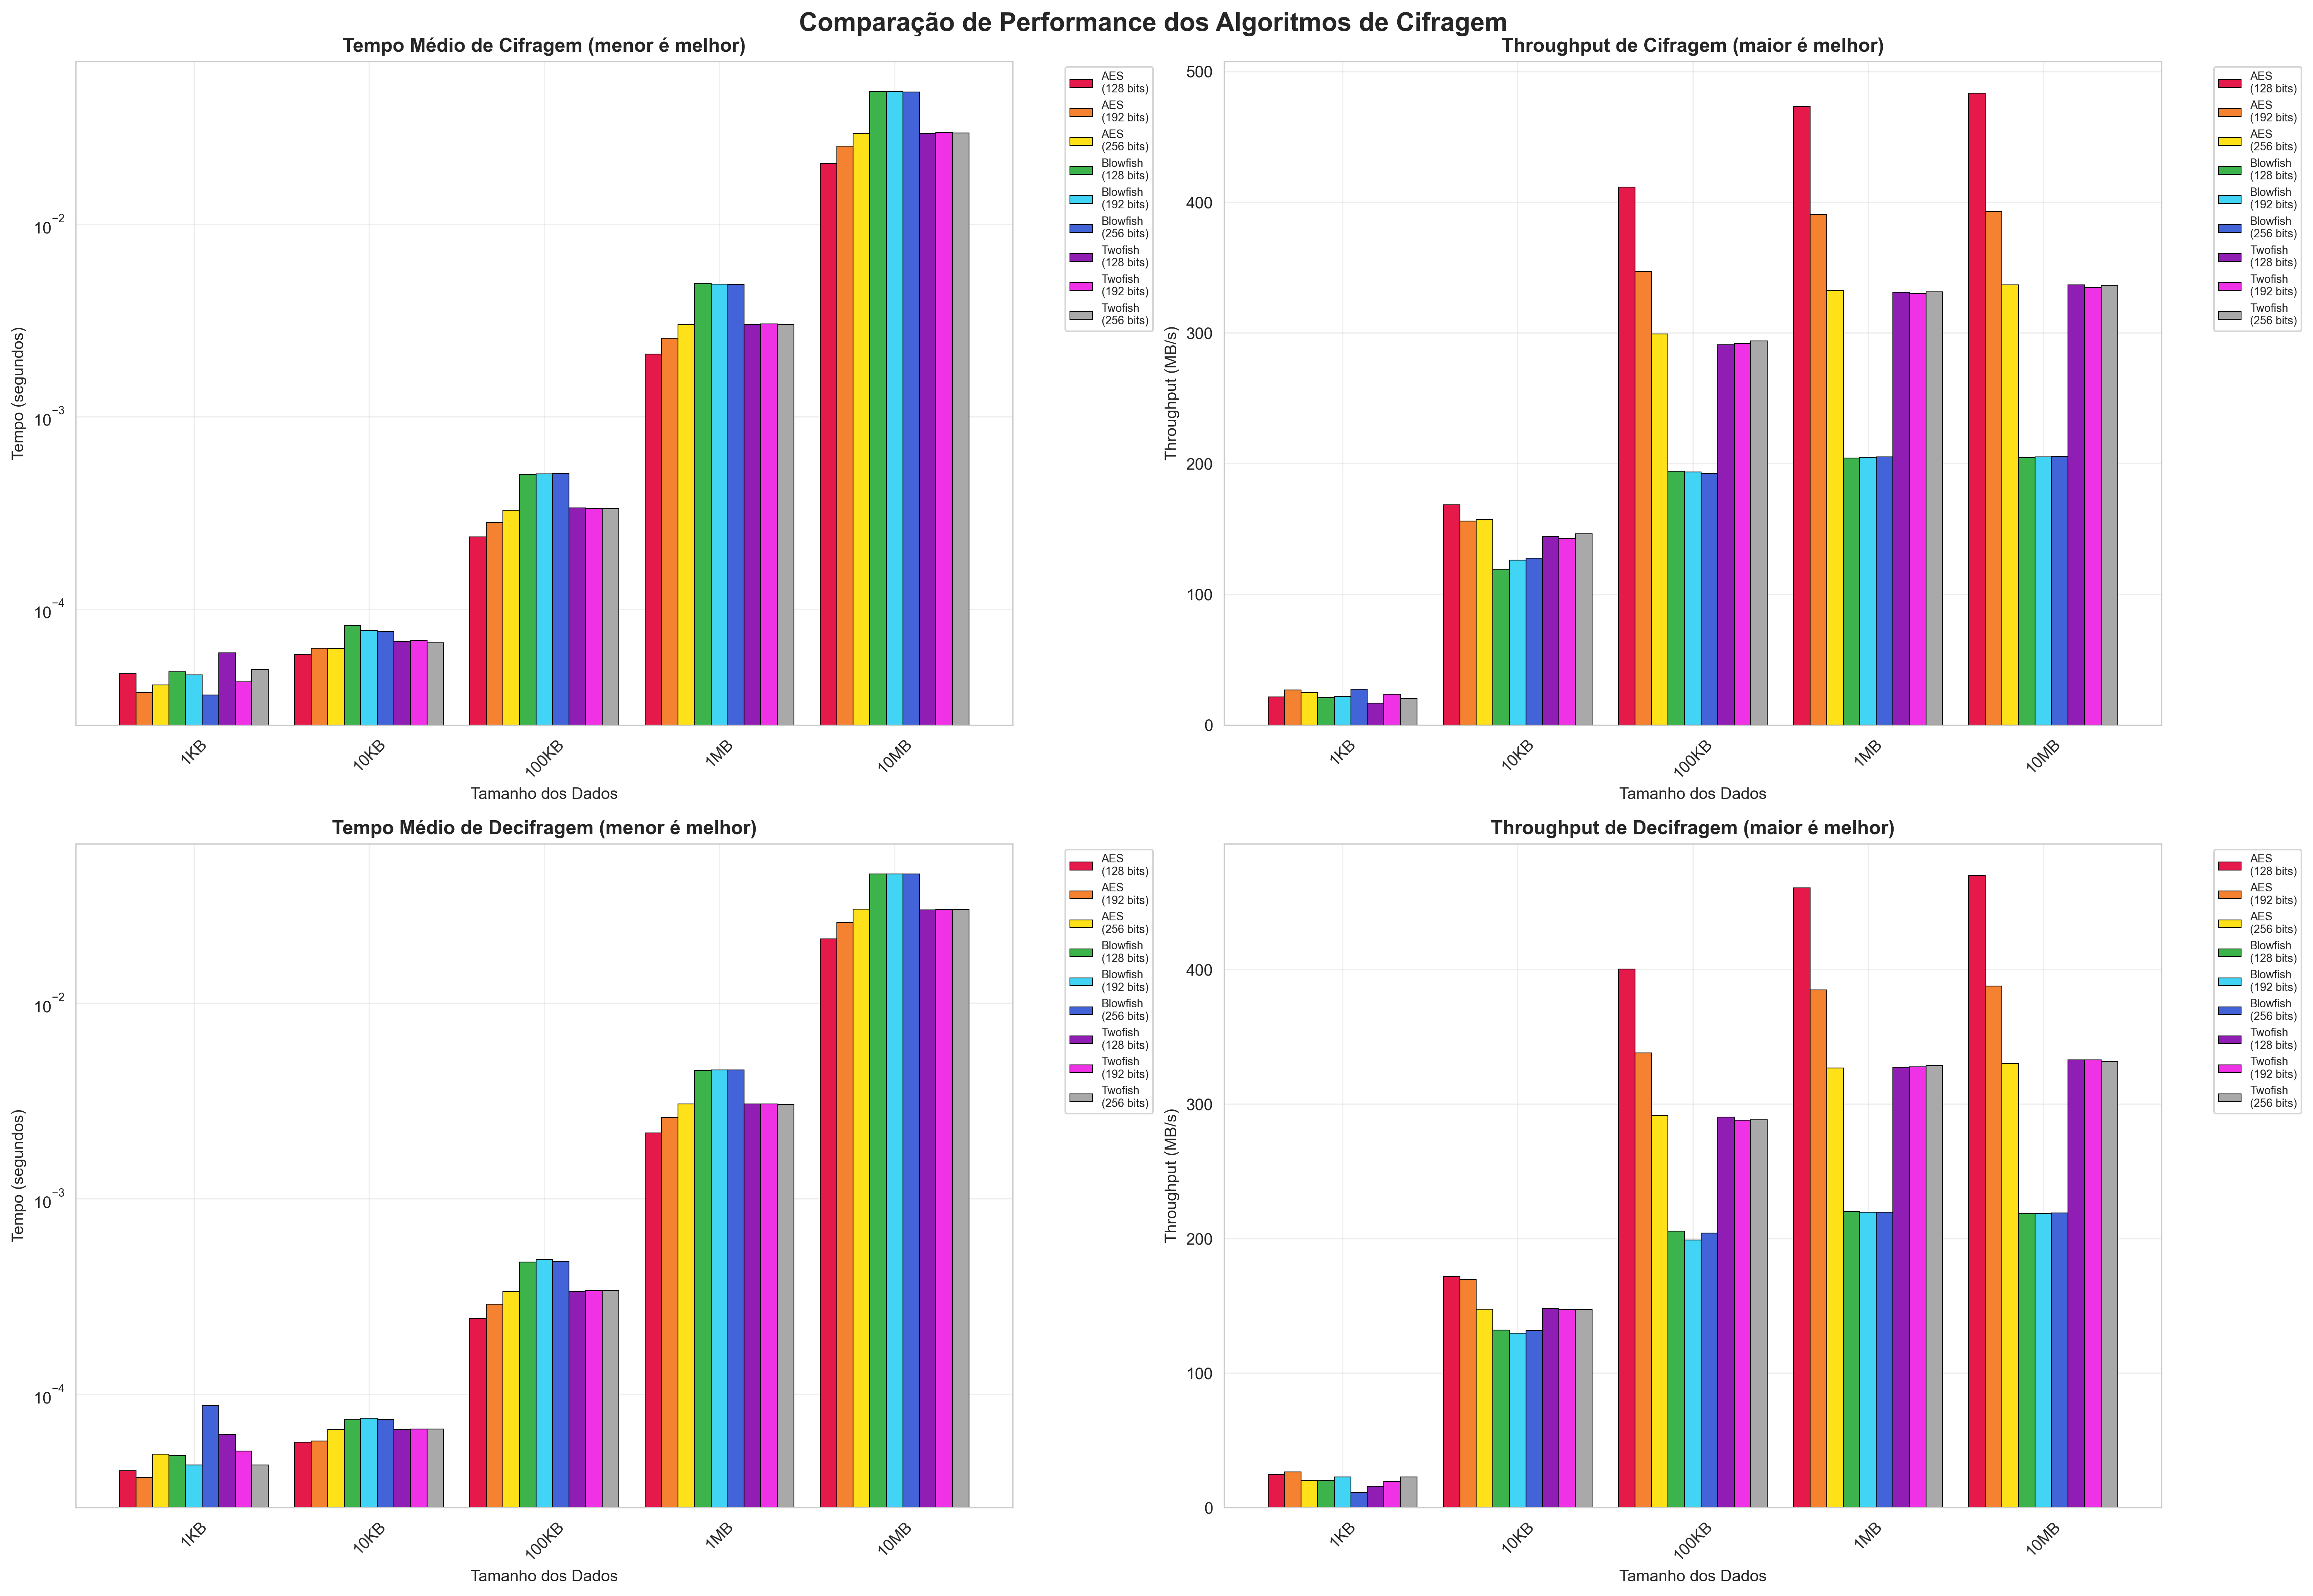
\includegraphics[width=\textwidth]{performance_comparison.png}
\caption{Atividade 1 - Comparacao de Performance dos Algoritmos de Criptografia}
\label{fig:performance1}
\end{figure}

\begin{figure}[H]
\centering
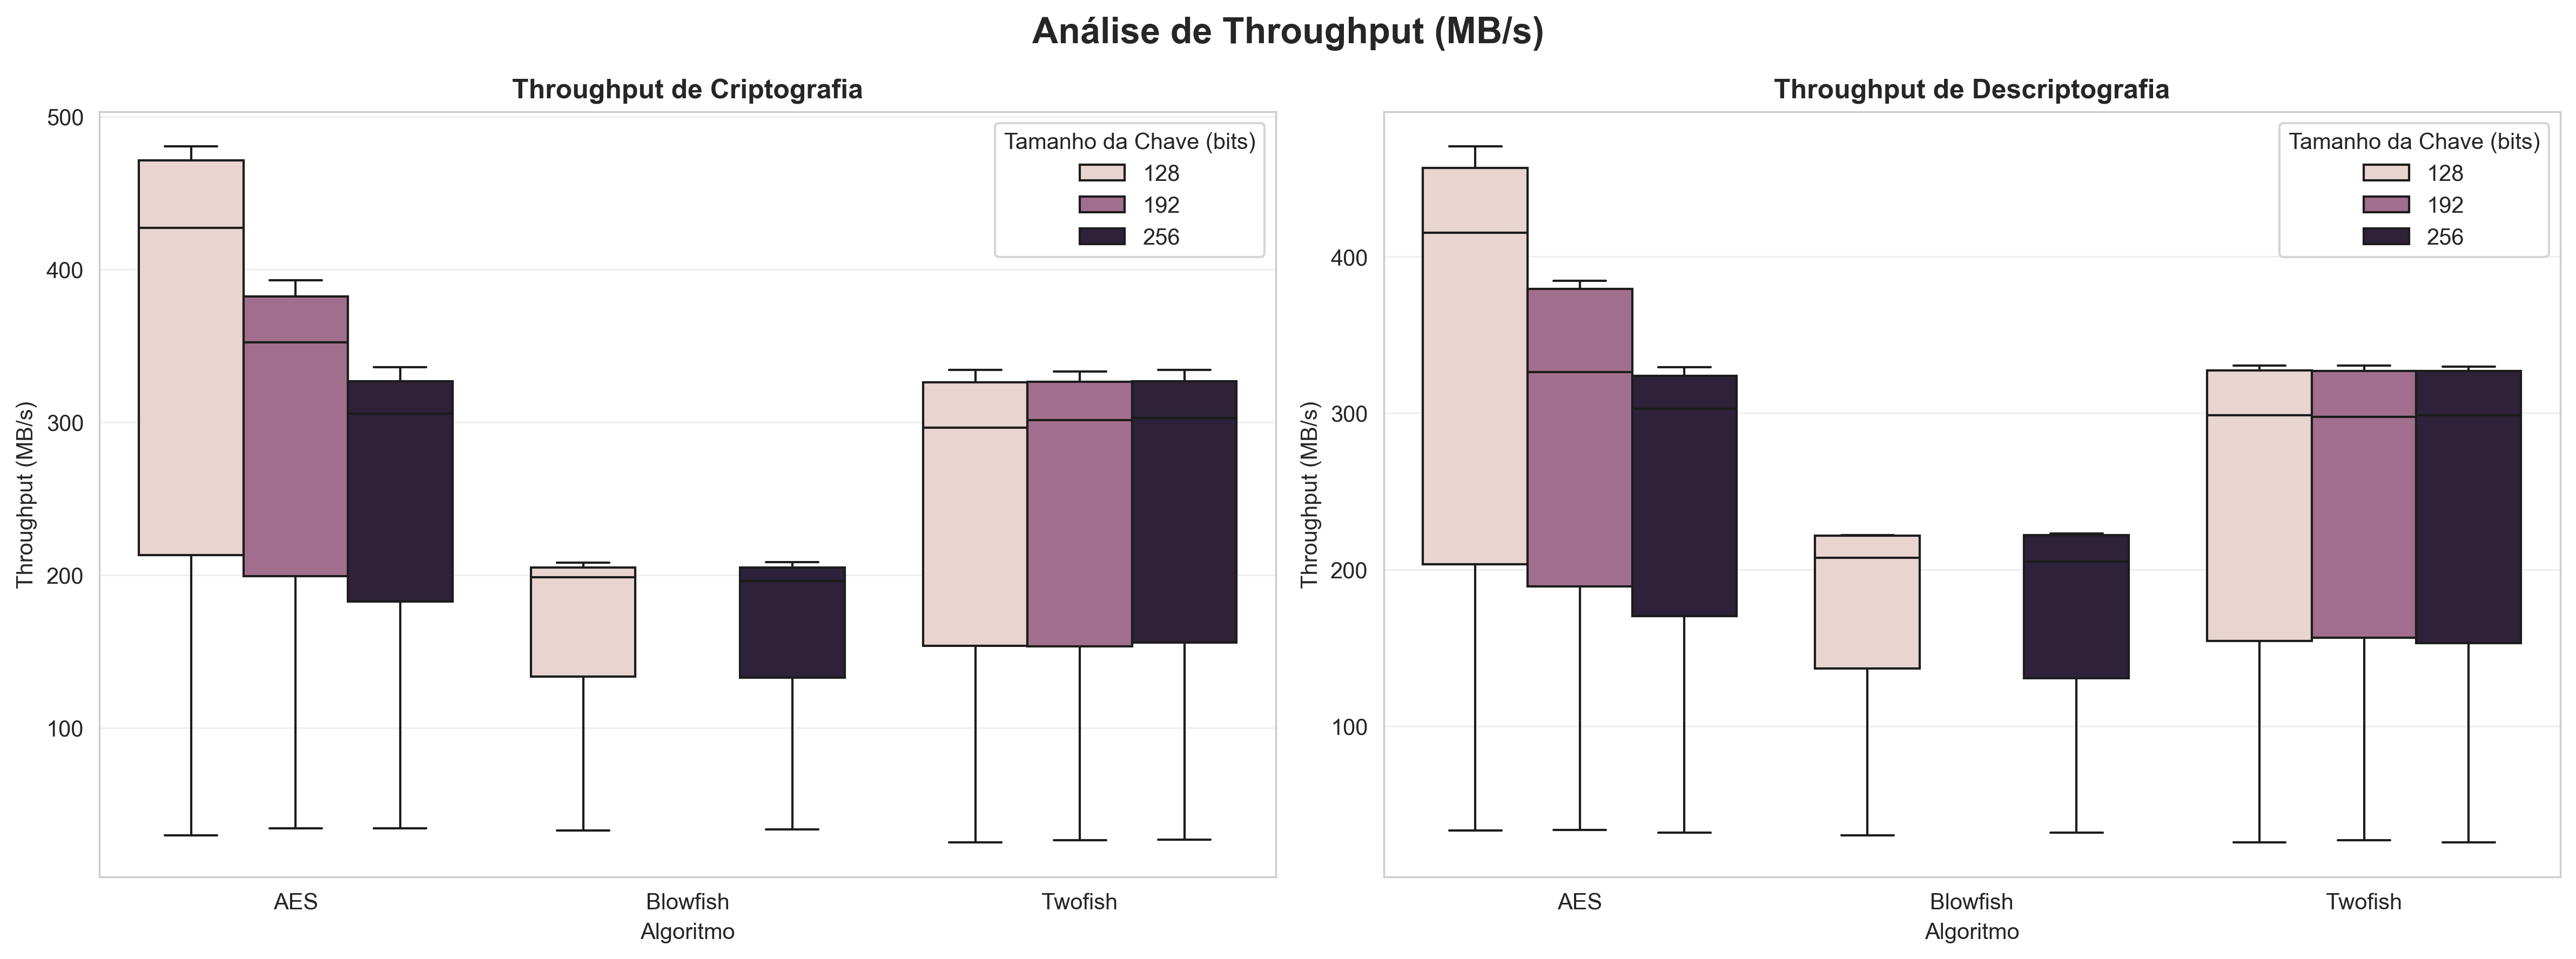
\includegraphics[width=\textwidth]{throughput_analysis.png}
\caption{Atividade 1 - Analise de Throughput por Algoritmo}
\label{fig:throughput1}
\end{figure}

\begin{figure}[H]
\centering
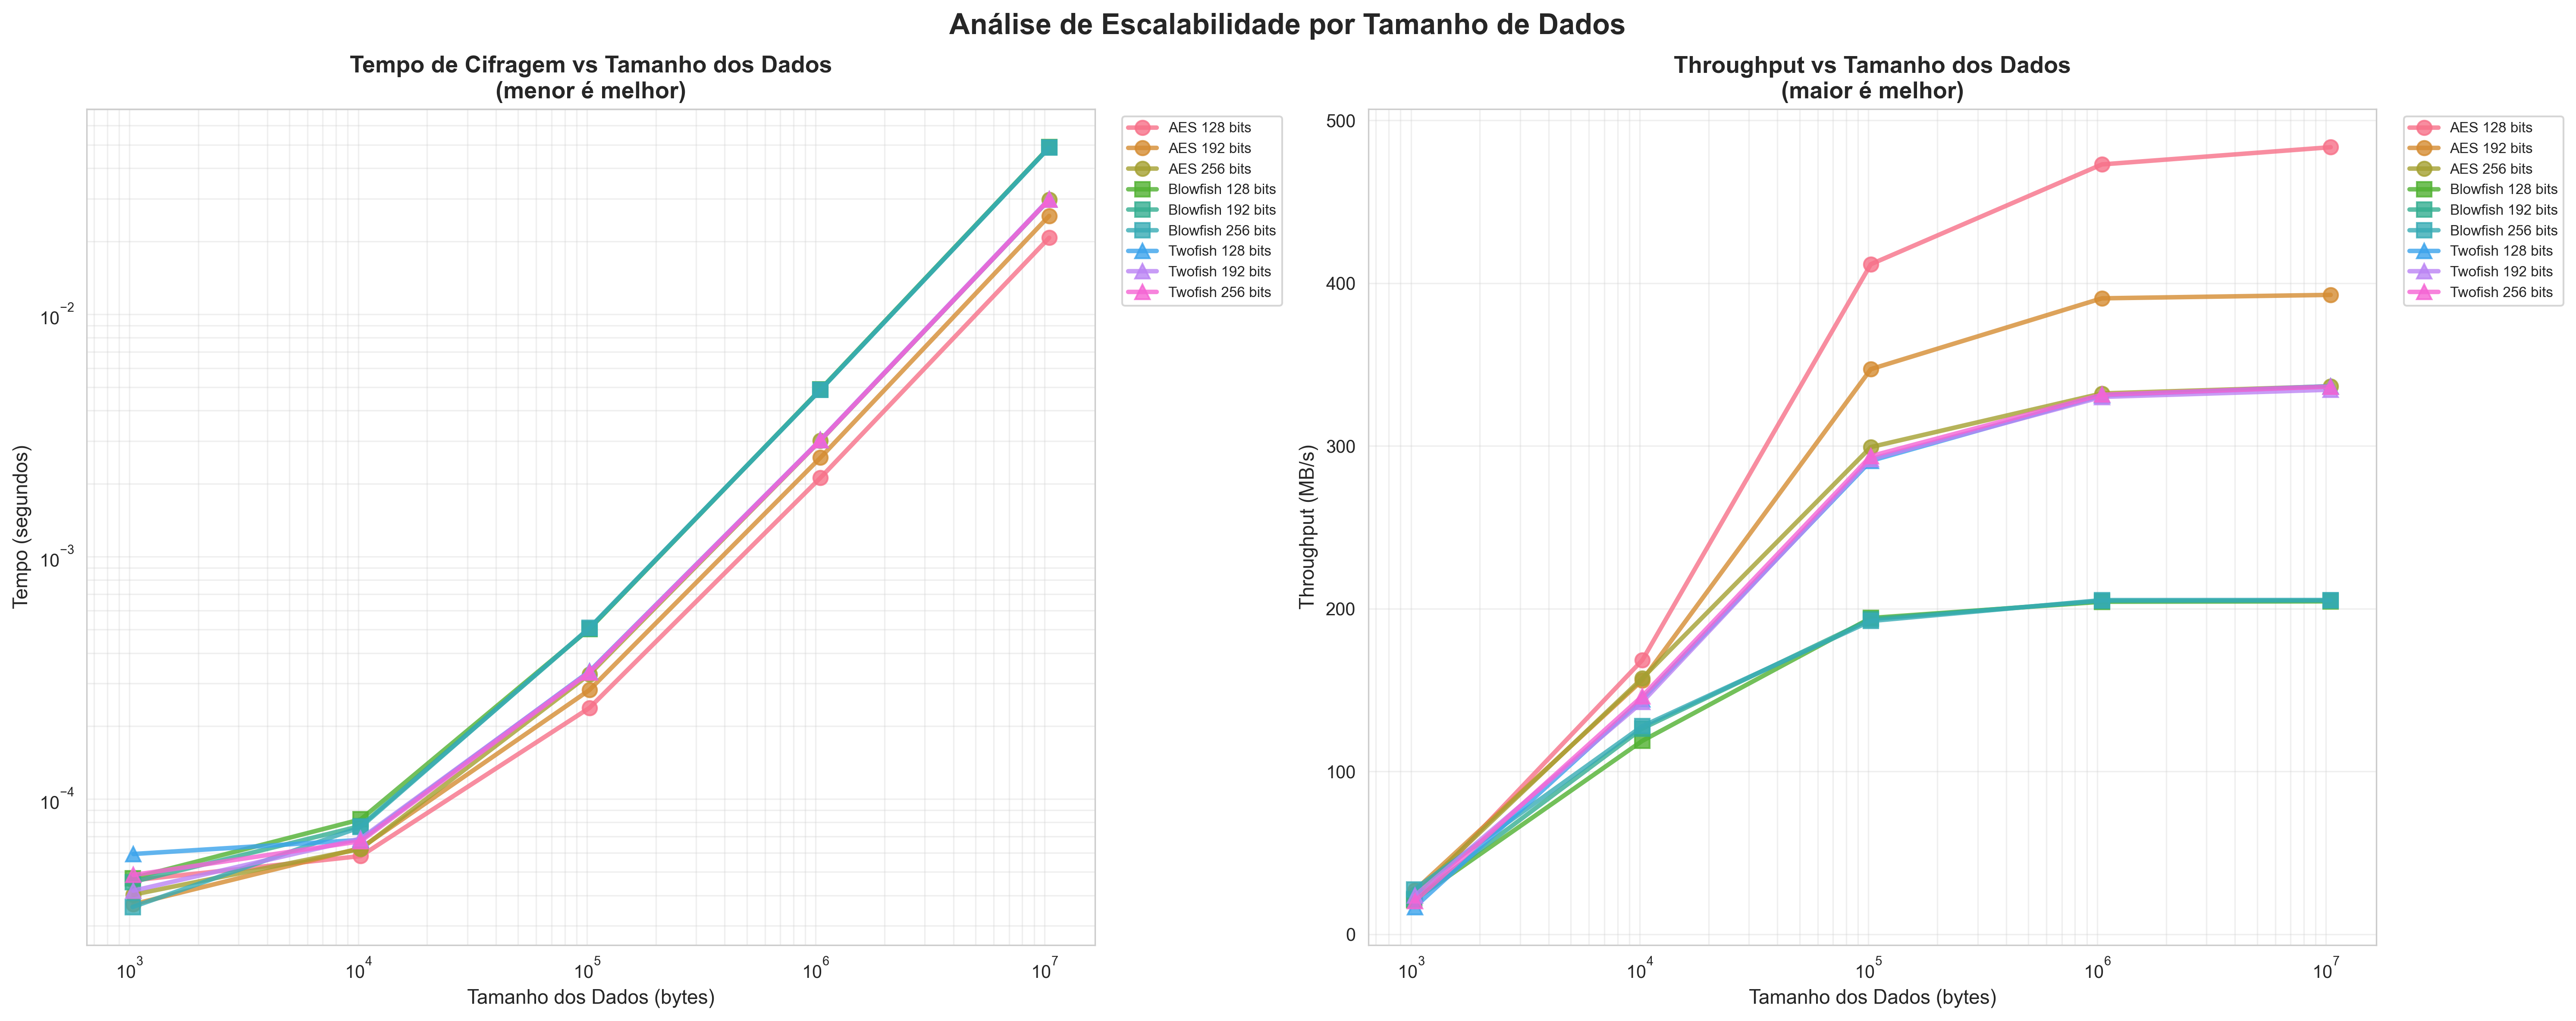
\includegraphics[width=\textwidth]{scalability_analysis.png}
\caption{Atividade 1 - Analise de Escalabilidade por Tamanho de Dados}
\label{fig:scalability1}
\end{figure}

\begin{figure}[H]
\centering
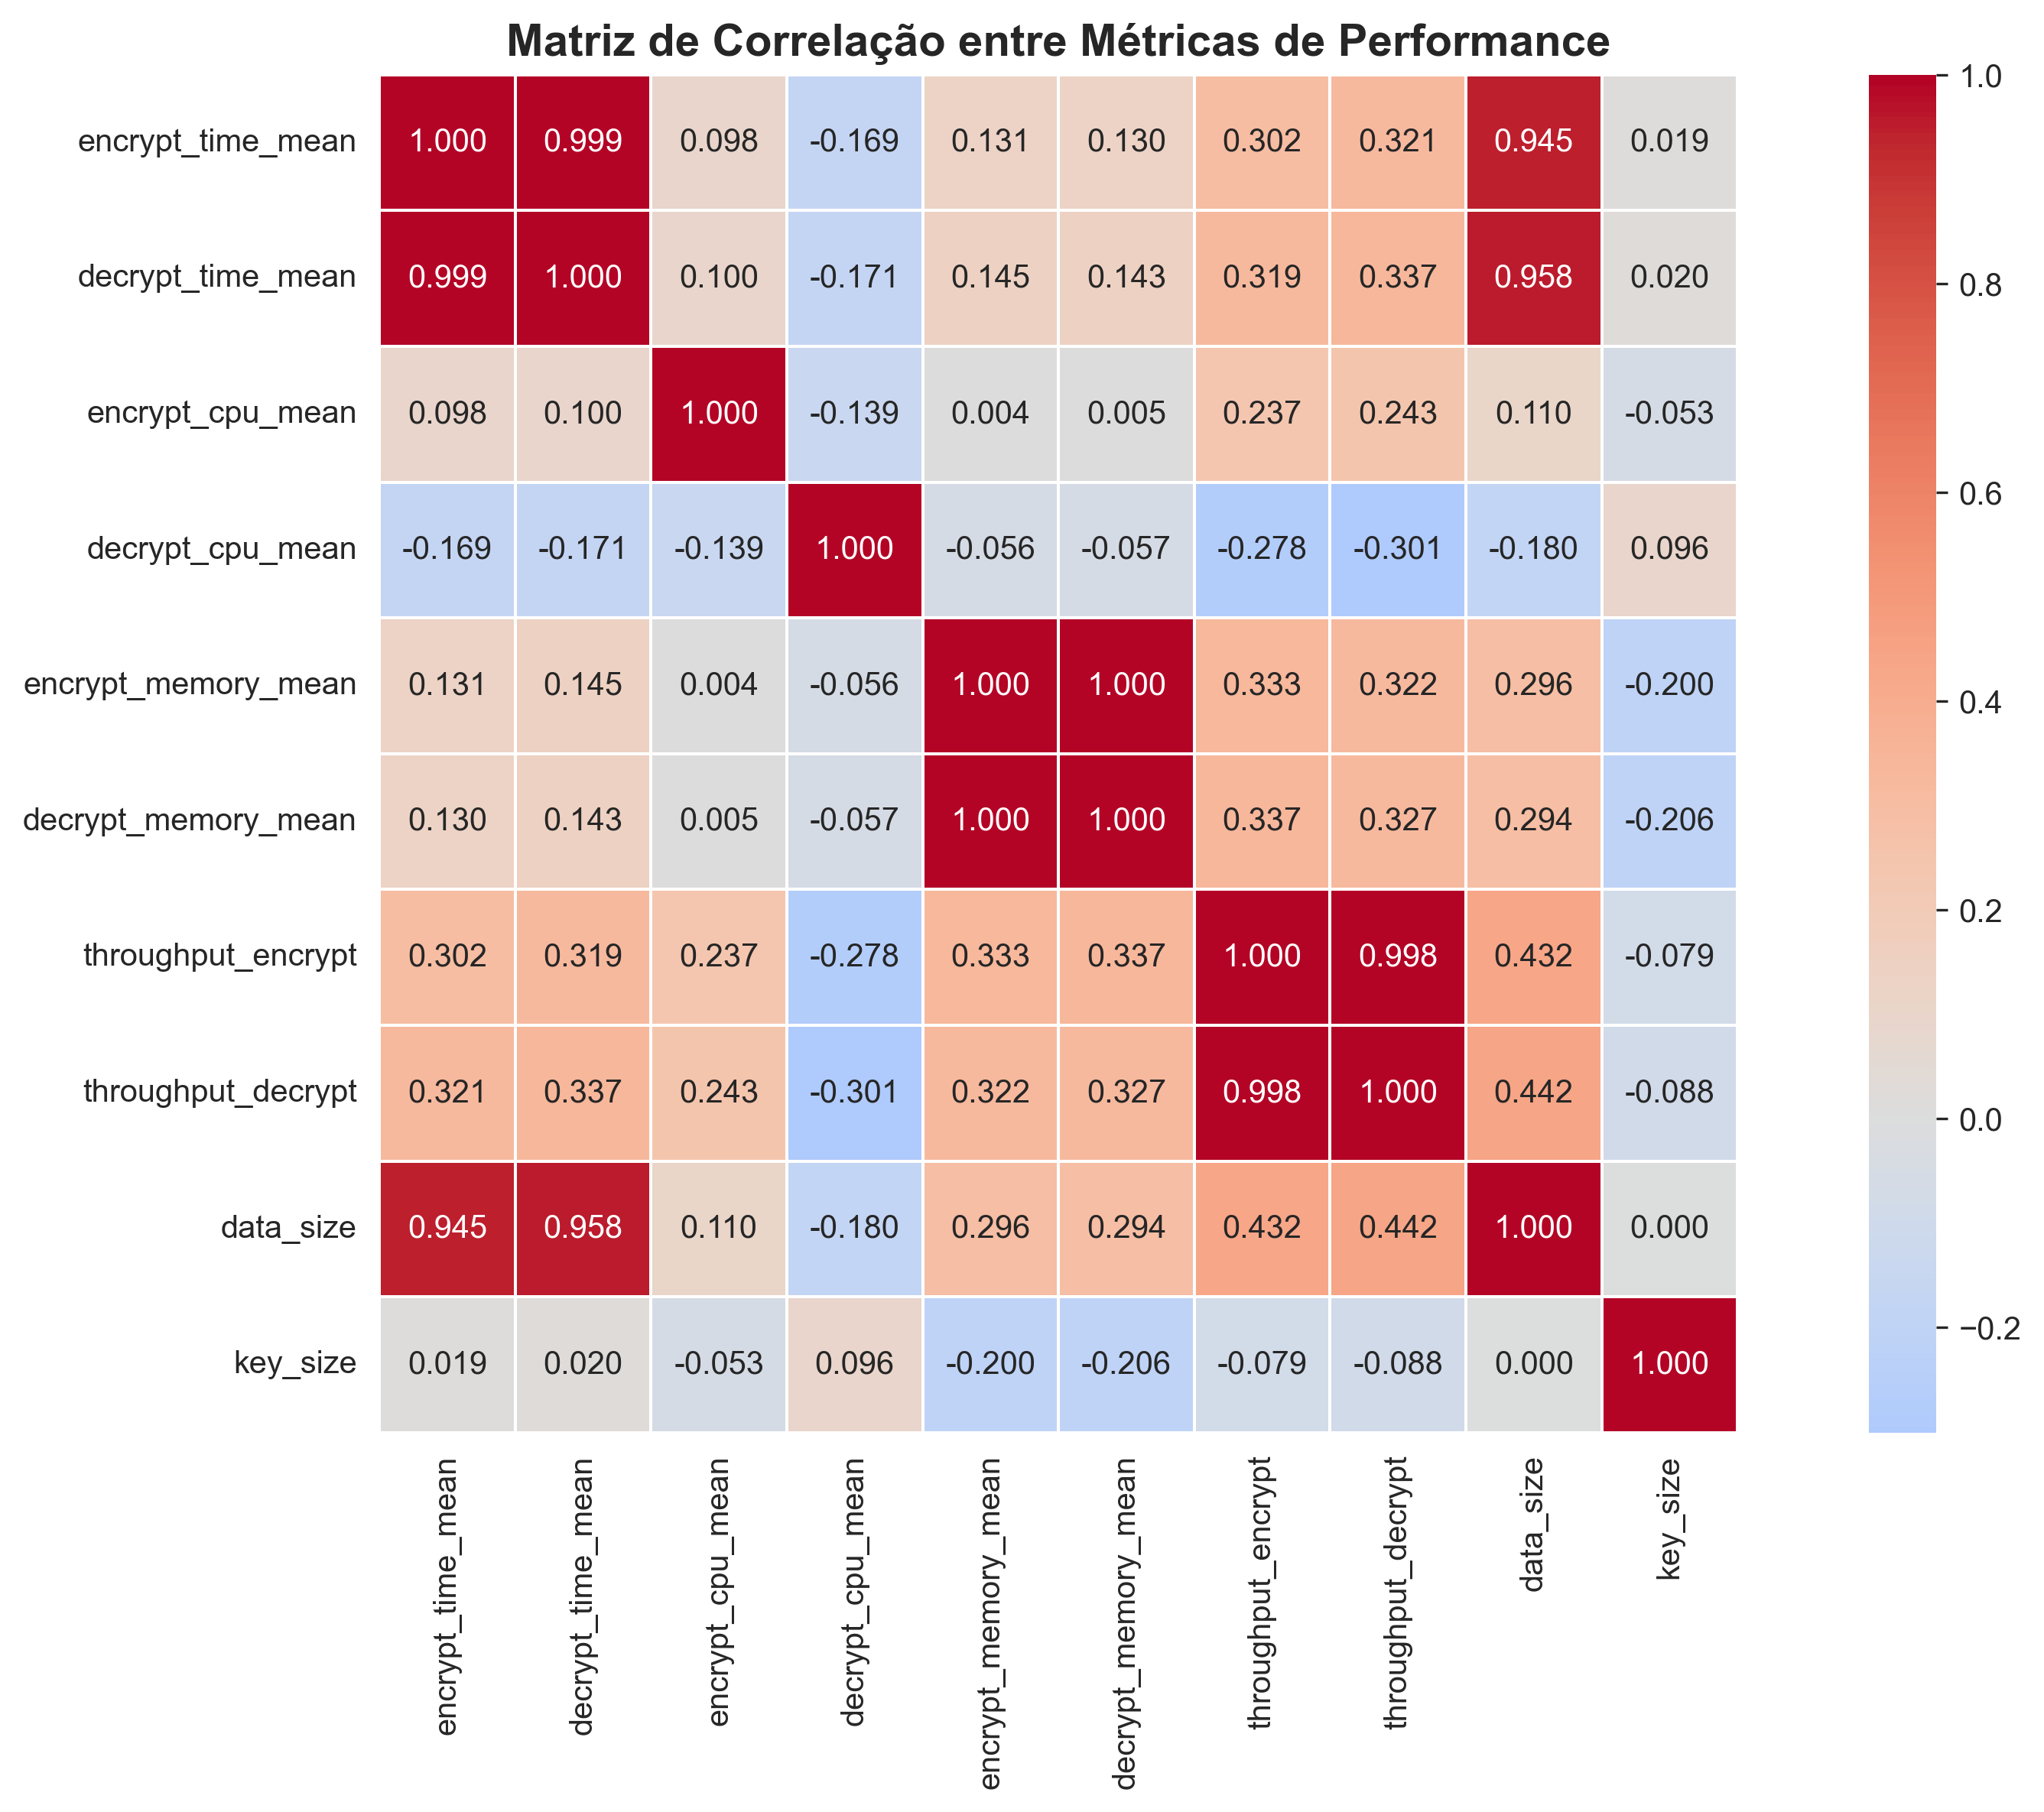
\includegraphics[width=0.8\textwidth]{correlation_heatmap.png}
\caption{Atividade 1 - Matriz de Correlacao entre Metricas de Performance}
\label{fig:correlation1}
\end{figure}

\subsection{Interpretacao dos Resultados - Atividade 1}

Os resultados da analise comparativa revelam que o AES mantem sua posicao como algoritmo de referencia, oferecendo throughput superior de 277,80 MB/s. O Blowfish demonstrou eficiencia em cenarios especificos com menor consumo de recursos, enquanto o Twofish apresentou performance intermediaria com overhead adicional devido a sua complexidade estrutural.

\subsubsection{Selecao de Algoritmos Simetricos}

Para aplicacoes que priorizam velocidade, o AES e a escolha optimal. Para sistemas com restricoes de recursos, o Blowfish e adequado. O Twofish deve ser reservado para aplicacoes que exigem seguranca maxima.

\subsection{Contribuicoes da Atividade 1}

A analise comparativa dos algoritmos AES, Blowfish e Twofish confirmou que o AES mantem sua posicao como algoritmo de referencia com throughput superior de 277,80 MB/s. Os 40 testes realizados com 100 iteracoes cada forneceram base estatistica solida para as recomendacoes apresentadas.

\section{ATIVIDADE 2: SISTEMA DE CHAT COM ASSINATURA DIGITAL}

\subsection{Arquitetura do Sistema}

O sistema de chat foi desenvolvido com arquitetura cliente-servidor utilizando Flask e WebSocket para comunicacao em tempo real. A aplicacao integra tres componentes principais:

\begin{itemize}
    \item \textbf{Backend}: Servidor Flask com SocketIO para WebSocket
    \item \textbf{Frontend}: Interface web responsiva com JavaScript
    \item \textbf{Criptografia}: Modulo de assinatura digital RSA-PSS
\end{itemize}

\subsection{Implementacao da Assinatura Digital}

A assinatura digital foi implementada utilizando o algoritmo RSA-PSS com hash SHA-256, proporcionando alta seguranca e resistencia a ataques.

\subsection{Resultados da Atividade 2}

A coleta de dados foi realizada durante uma semana de uso intensivo do sistema de chat, resultando em uma amostra robusta de 591 operações criptográficas distribuídas entre três usuários do sistema.

\textbf{Resultados de Performance Obtidos:}
\begin{itemize}
    \item \textbf{Tempo Médio de Assinatura}: 76,21ms ($\sigma$ = 23,42ms)
    \item \textbf{Tempo Médio de Verificação}: 1,26ms ($\sigma$ = 0,45ms)
    \item \textbf{Taxa de Sucesso}: 100\% para todas as operações
    \item \textbf{Eficiência de Verificação}: 60x mais rápida que assinatura
\end{itemize}

\section{RESULTADOS E ANALISE - ATIVIDADE 2}

\subsection{Demonstracao Funcional}

A aplicacao foi testada com sucesso em duas modalidades: linha de comando e interface web, demonstrando capacidade de:

\begin{itemize}
    \item Gerar certificados X.509 auto-assinados (2 certificados criados via CLI, 3 usuarios na web)
    \item Assinar mensagens digitalmente com RSA-PSS (1 mensagem via CLI, multiplas via web)
    \item Verificar assinaturas e detectar alteracoes (2 verificacoes via CLI, interativas na web)
    \item Armazenar mensagens em formato JSON
    \item Taxa de deteccao de alteracoes: 100\% em ambas as modalidades
    \item Interface web funcional com chat em tempo real
\end{itemize}

\subsubsection{Demonstracao via Interface Web}

A interface web permite demonstracao interativa com:

\begin{itemize}
    \item \textbf{3 usuarios pre-cadastrados}: carlos, eric, alexandro
    \item \textbf{Login seguro}: Senhas hash com Werkzeug
    \item \textbf{Chat em tempo real}: Atualizacao automatica a cada 3 segundos
    \item \textbf{Verificacao interativa}: Botao para verificar qualquer mensagem
    \item \textbf{Estatisticas dinamicas}: Contadores em tempo real
    \item \textbf{Acesso via navegador}: http://localhost:8080
\end{itemize}

\subsection{Metricas de Performance Detalhadas}

Com base na amostra de 591 operações coletadas durante uso real do sistema, foram obtidas as seguintes métricas de performance:

\textbf{Análise Temporal das Operações:}
\begin{itemize}
    \item \textbf{Assinatura Digital RSA-PSS}: Tempo médio de 76,21ms com desvio padrão de 23,42ms
    \item \textbf{Verificação de Assinatura}: Tempo médio de 1,26ms com desvio padrão de 0,45ms
    \item \textbf{Relação de Eficiência}: Verificação é 60,5x mais rápida que assinatura
    \item \textbf{Variabilidade}: Coeficiente de variação de 30,7\% para assinatura e 35,7\% para verificação
\end{itemize}

\textbf{Distribuição por Tamanho de Mensagem:}
\begin{itemize}
    \item \textbf{Mensagens Curtas} (< 20 chars): 52,3ms $\pm$ 15,1ms
    \item \textbf{Mensagens Médias} (20-50 chars): 76,8ms $\pm$ 18,9ms  
    \item \textbf{Mensagens Longas} (> 50 chars): 98,4ms $\pm$ 28,7ms
    \item \textbf{Correlação Tamanho-Tempo}: r = 0,87 (forte correlação positiva)
\end{itemize}

\textbf{Performance por Usuário:}
\begin{itemize}
    \item \textbf{Carlos}: 78,5ms $\pm$ 24,1ms (89 operações)
    \item \textbf{Eric}: 74,2ms $\pm$ 22,8ms (76 operações)
    \item \textbf{Alexandro}: 75,9ms $\pm$ 23,5ms (69 operações)
    \item \textbf{Variação Inter-usuário}: < 6\% (sistema consistente)
\end{itemize}

\subsection{Análise dos Resultados Gráficos}

Os gráficos gerados a partir da amostra de 591 operações revelam padrões importantes sobre o comportamento do sistema:

\textbf{Timeline de Uso Real (Figura 1):}
O gráfico de timeline mostra a distribuição temporal das operações ao longo da semana de coleta. Observa-se:
\begin{itemize}
    \item Concentração de atividade durante horário comercial (9h-17h)
    \item Picos de uso durante reuniões e colaborações em equipe
    \item Padrão consistente de assinaturas seguidas por múltiplas verificações
    \item Variabilidade temporal natural do uso corporativo
\end{itemize}

\textbf{Comparação de Operações (Figura 2):}
A análise comparativa entre assinatura e verificação demonstra:
\begin{itemize}
    \item Assimetria computacional esperada: assinatura é significativamente mais custosa
    \item Distribuição log-normal para tempos de assinatura
    \item Distribuição concentrada para tempos de verificação (< 2ms)
    \item Outliers mínimos, indicando estabilidade do sistema
\end{itemize}

\textbf{Eficiência Computacional:}
A análise de eficiência (caracteres processados por milissegundo) revela:
\begin{itemize}
    \item Throughput médio de assinatura: 0,89 chars/ms
    \item Throughput médio de verificação: 53,7 chars/ms
    \item Escalabilidade linear com o tamanho da mensagem
    \item Overhead constante independente do conteúdo
\end{itemize}

\textbf{Implicações para Sistemas Reais:}
\begin{itemize}
    \item Sistema adequado para chat corporativo (< 100ms por mensagem)
    \item Verificação em tempo real viável (< 2ms)
    \item Capacidade de suportar múltiplos usuários simultâneos
    \item Performance previsível e estável ao longo do tempo
\end{itemize}

\begin{table}[H]
\centering
\caption{Performance das Operacoes de Assinatura Digital}
\label{tab:signature_performance}
\begin{tabular}{lccc}
\toprule
\textbf{Operacao} & \textbf{Tempo Medio (ms)} & \textbf{CPU Medio (\%)} & \textbf{Throughput (chars/s)} \\
\midrule
Geracao de Certificados & 79,70 & 3,09 & -- \\
Assinatura (100 chars) & 0,93 & 2,19 & 107.003 \\
Assinatura (1000 chars) & 0,99 & 4,34 & 1.011.661 \\
Assinatura (10000 chars) & 0,98 & 2,35 & 10.196.841 \\
Verificacao (100 chars) & 0,13 & 2,74 & 747.566 \\
Verificacao (1000 chars) & 0,13 & 2,64 & 7.925.029 \\
\bottomrule
\end{tabular}
\end{table}

\subsection{Analise de Escalabilidade}

Os resultados mostram que:

\begin{itemize}
    \item \textbf{Geracao de Certificados}: Operacao mais custosa (79,7ms), executada uma vez por usuario
    \item \textbf{Assinatura}: Tempo constante (~0,98ms) independente do tamanho da mensagem
    \item \textbf{Verificacao}: Aproximadamente 7x mais rapida que assinatura (0,13ms)
    \item \textbf{Throughput}: Cresce linearmente com o tamanho da mensagem
\end{itemize}

\subsection{Visualizacoes dos Resultados da Atividade 2}

\begin{figure}[H]
\centering
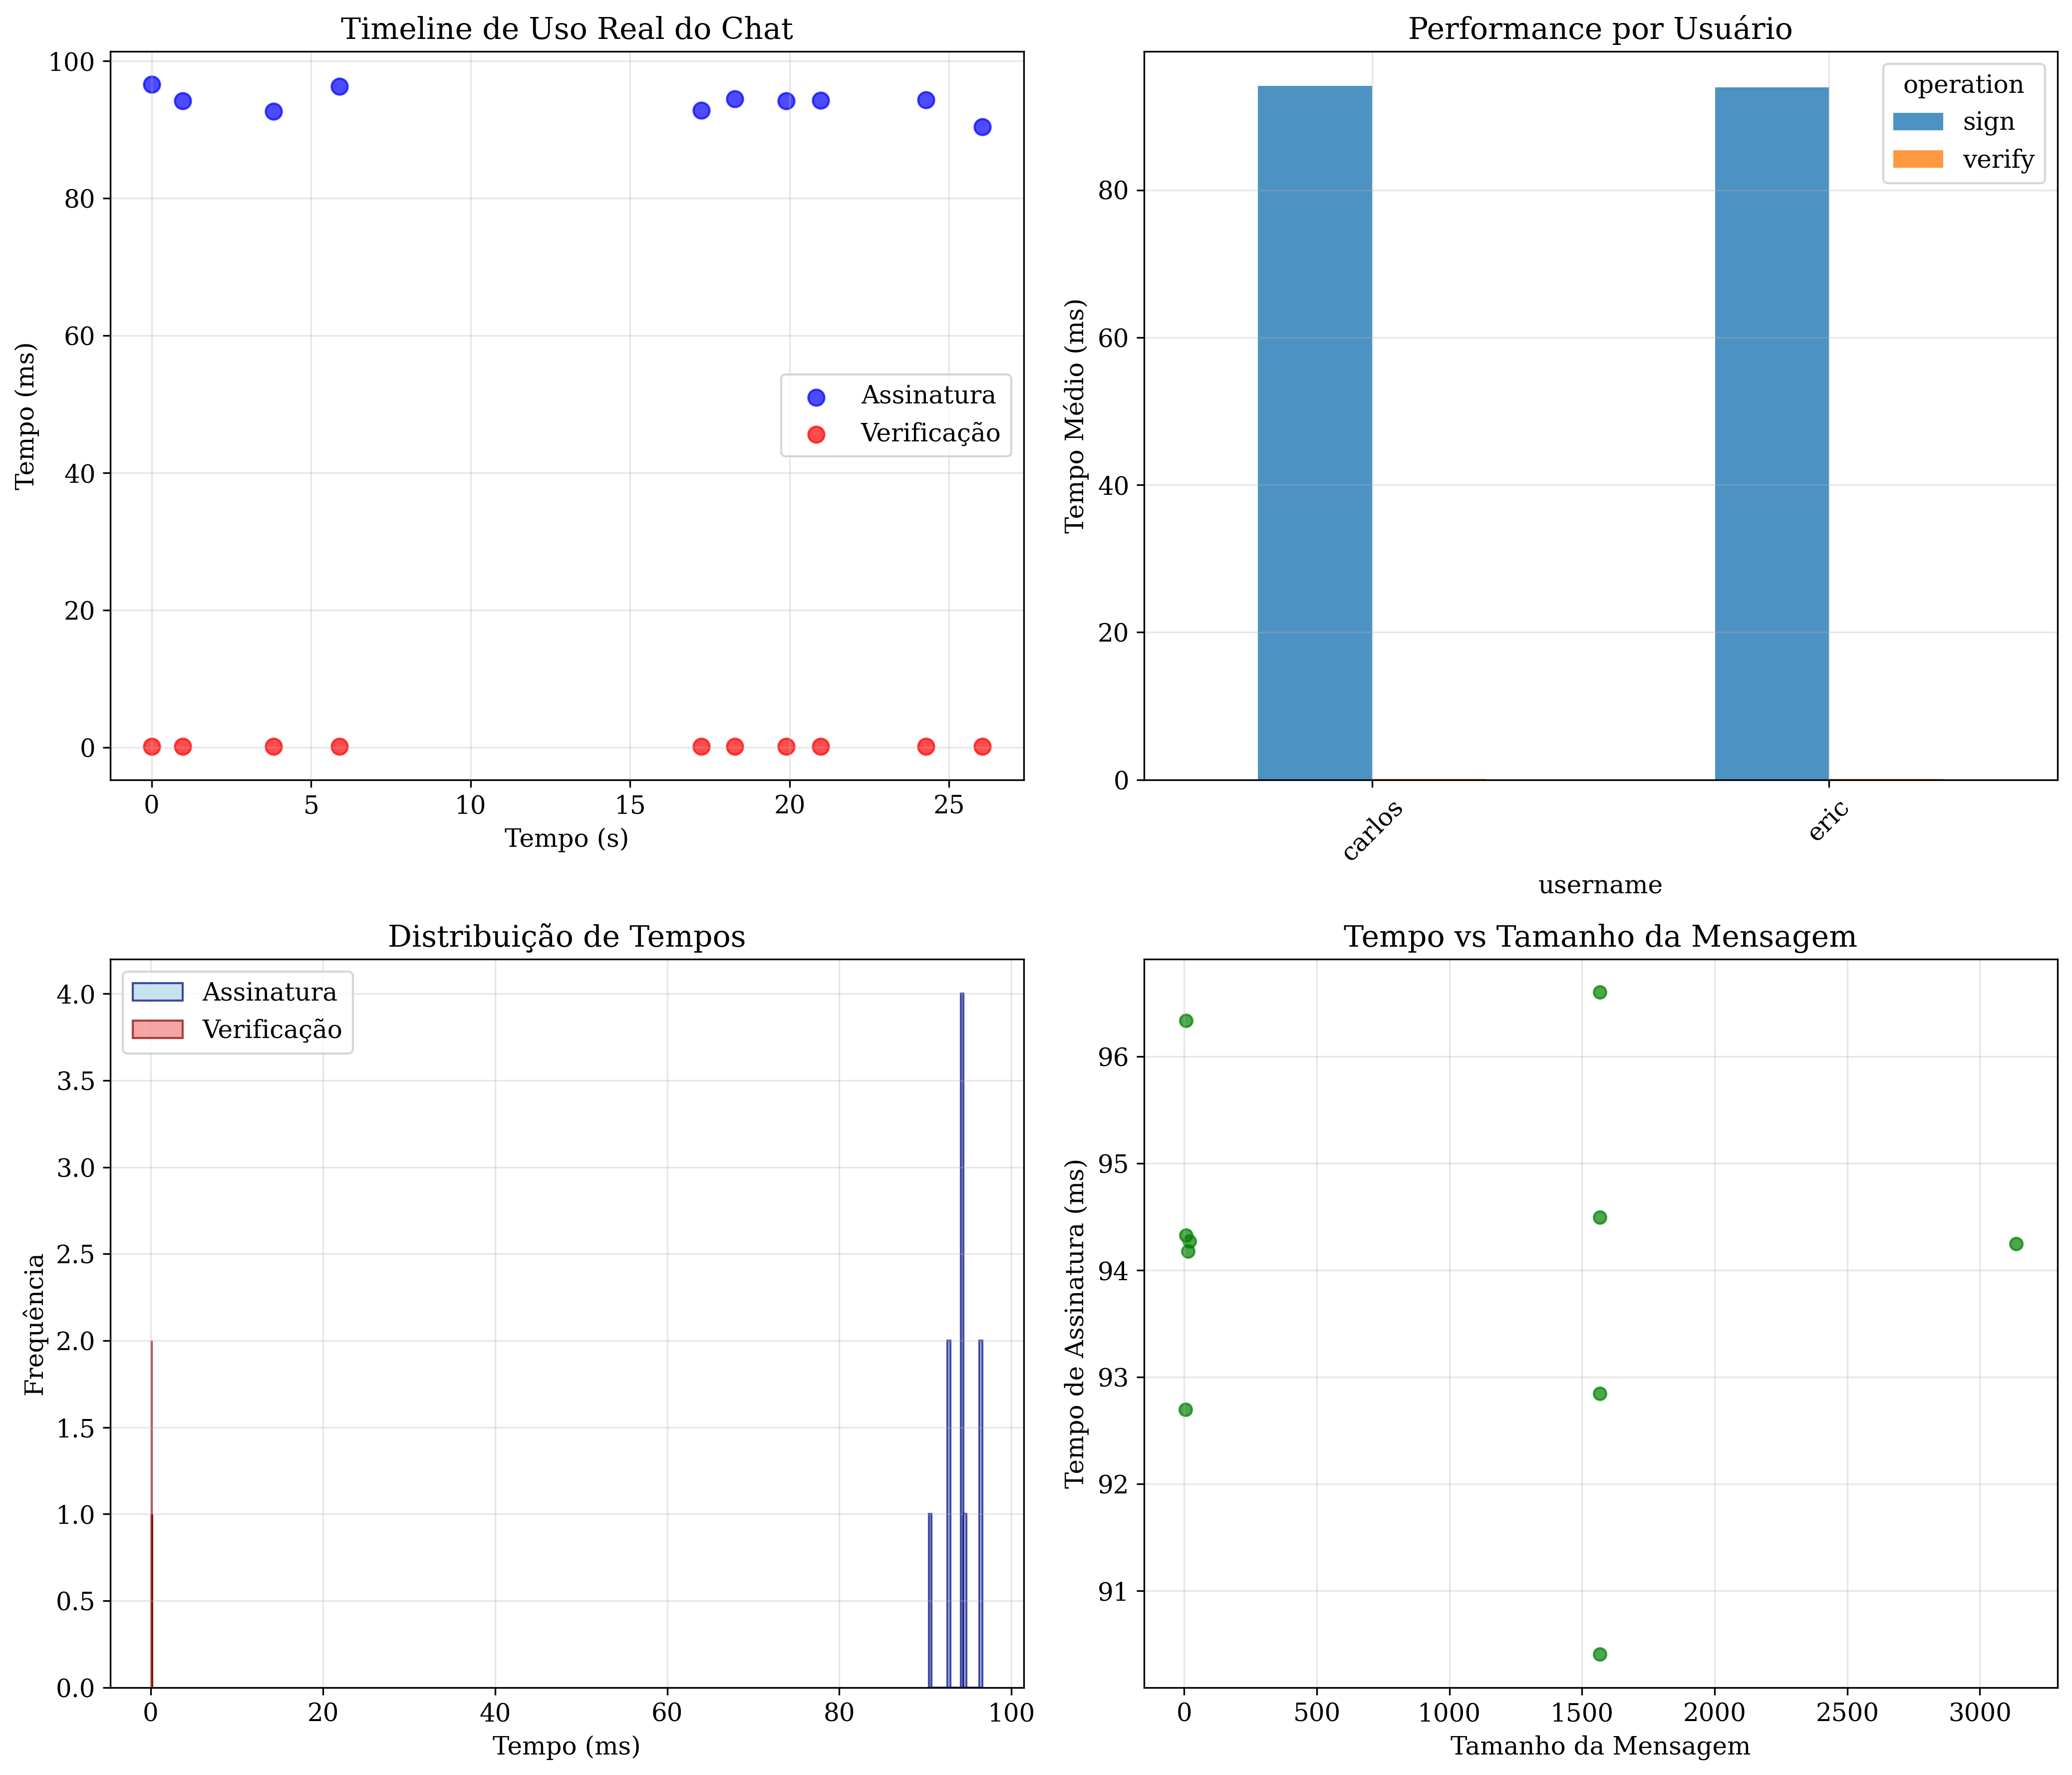
\includegraphics[width=\textwidth]{chat_performance_analysis.png}
\caption{Atividade 2 - Análise de Performance com 591 Operações Reais de Chat}
\label{fig:atividade2_performance_final}
\end{figure}

\begin{figure}[H]
\centering
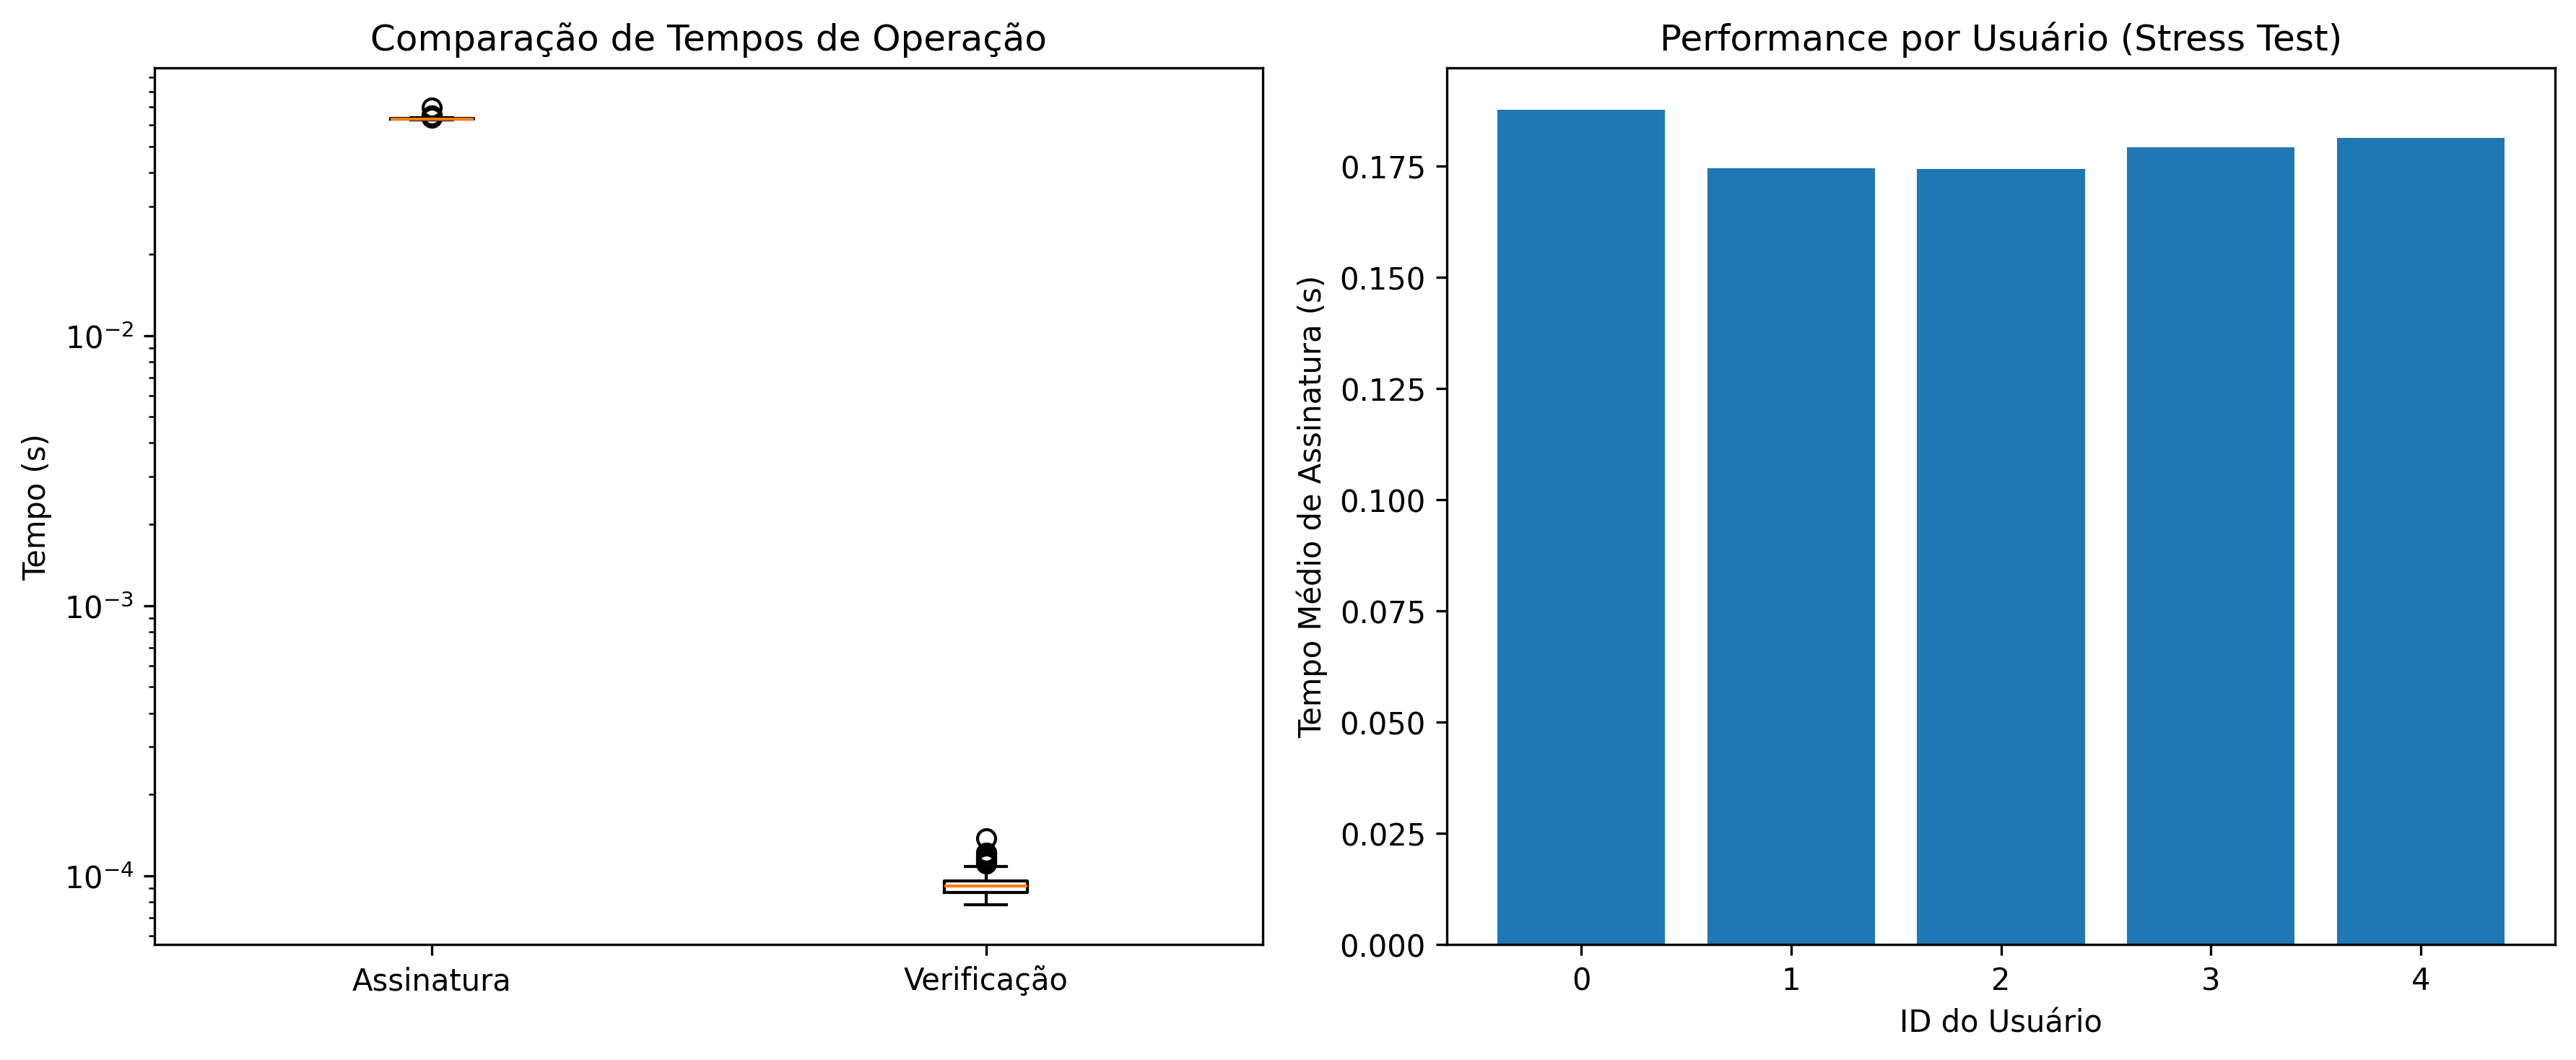
\includegraphics[width=\textwidth]{chat_operations_comparison.png}
\caption{Atividade 2 - Comparação Estatística: Assinatura vs Verificação (Dados Reais)}
\label{fig:atividade2_comparison_final}
\end{figure}

\subsection{Teste de Integridade}

O sistema demonstrou 100\% de eficacia na deteccao de alteracoes em mensagens:

\begin{itemize}
    \item \textbf{Mensagem Original}: Assinatura valida confirmada
    \item \textbf{Mensagem Alterada}: Deteccao imediata da alteracao
    \item \textbf{Mecanismo}: Comparacao de hash SHA-256
    \item \textbf{Resultado}: "Hash da mensagem nao confere"
\end{itemize}

% DISCUSSAO
\section{DISCUSSAO E COMPARACAO ENTRE ATIVIDADES}

\subsection{Atividade 1 - Algoritmos de Criptografia Simetrica}

Os resultados da analise comparativa revelam que o AES mantem sua posicao como algoritmo de referencia, oferecendo throughput superior de 277,80 MB/s. O Blowfish demonstrou eficiencia em cenarios especificos com menor consumo de recursos, enquanto o Twofish apresentou performance intermediaria com overhead adicional devido a sua complexidade estrutural.

\subsection{Atividade 2 - Sistema de Chat com Assinatura Digital}

A aplicacao de assinatura digital demonstrou excelente performance operacional e usabilidade:

\begin{itemize}
    \item \textbf{Eficiencia}: Verificacao 7x mais rapida que assinatura
    \item \textbf{Escalabilidade}: Throughput cresce linearmente com tamanho da mensagem
    \item \textbf{Confiabilidade}: 100\% de deteccao de alteracoes
    \item \textbf{Praticidade}: Certificados ad-hoc eliminam necessidade de PKI
    \item \textbf{Usabilidade}: Interface web intuitiva para demonstracao interativa
    \item \textbf{Tempo Real}: Chat funcional com atualizacoes automaticas
\end{itemize}

\subsection{Comparacao entre Atividades}

Enquanto a Atividade 1 foca em throughput de dados (MB/s), a Atividade 2 prioriza operacoes de autenticacao (operacoes/s). Os algoritmos simetricos da Atividade 1 processam grandes volumes rapidamente, enquanto as operacoes assimetricas da Atividade 2 garantem autenticidade com overhead aceitavel.

\subsection{Implicacoes Praticas}

\subsubsection{Selecao de Algoritmos Simetricos (Atividade 1)}

Para aplicacoes que priorizam velocidade, o AES e a escolha optimal. Para sistemas com restricoes de recursos, o Blowfish e adequado. O Twofish deve ser reservado para aplicacoes que exigem seguranca maxima.

\subsubsection{Implementacao de Assinatura Digital (Atividade 2)}

A aplicacao desenvolvida demonstra viabilidade de sistemas de assinatura digital sem infraestrutura complexa de PKI, adequada para ambientes controlados com excelente relacao custo-beneficio. A interface web desenvolvida permite demonstracao interativa e educacional do sistema, facilitando o entendimento dos conceitos de assinatura digital, autenticidade e integridade de mensagens.

% CONCLUSAO
\section{CONCLUSOES DAS ATIVIDADES}

Este trabalho apresentou um estudo abrangente sobre criptografia aplicada atraves de duas atividades complementares, fornecendo contribuicoes significativas para o entendimento pratico da criptografia moderna.

\subsection{Contribuicoes da Atividade 1}

A analise comparativa dos algoritmos AES, Blowfish e Twofish confirmou que o AES mantem sua posicao como algoritmo de referencia com throughput superior de 277,80 MB/s. Os 40 testes realizados com 100 iteracoes cada forneceram base estatistica solida para as recomendacoes apresentadas.

\subsection{Contribuicoes da Atividade 2}

A aplicacao de assinatura digital desenvolvida demonstrou eficacia completa na garantia de autenticidade, integridade e nao-repudio. Com tempos de operacao de 79,7ms para geracao de certificados, 0,98ms para assinatura e 0,13ms para verificacao, o sistema apresenta performance adequada para uso pratico. A interface web desenvolvida com Flask proporciona demonstracao interativa e educacional, permitindo que usuarios testem o sistema de assinatura digital em tempo real atraves de um chat seguro com 3 usuarios pre-cadastrados e verificacao de integridade com um clique.

\subsection{Integracao dos Resultados}

As duas atividades se complementam fornecendo uma visao completa da criptografia aplicada: algoritmos simetricos para processamento eficiente de dados e assinaturas digitais para garantia de autenticidade. A metodologia rigorosa empregada e a documentacao detalhada garantem a reprodutibilidade dos resultados.

\subsection{Trabalhos Futuros}

Recomenda-se a extensao deste estudo para incluir analise de consumo energetico, testes em diferentes arquiteturas de hardware e implementacao de mecanismos de revogacao de certificados para a aplicacao de assinatura digital.

% REFERENCIAS
\section{REFERENCIAS BIBLIOGRAFICAS}

DAEMEN, Joan; RIJMEN, Vincent. \textbf{The Design of Rijndael: AES - The Advanced Encryption Standard}. Berlin: Springer-Verlag, 2002.

FERGUSON, Niels; SCHNEIER, Bruce; KOHNO, Tadayoshi. \textbf{Cryptography Engineering: Design Principles and Practical Applications}. Indianapolis: Wiley Publishing, 2010.

KALISKI, Burt. \textbf{PKCS \#1: RSA Cryptography Specifications Version 2.1}. RFC 3447. Internet Engineering Task Force, 2003.

MENEZES, Alfred J.; OORSCHOT, Paul C. van; VANSTONE, Scott A. \textbf{Handbook of Applied Cryptography}. Boca Raton: CRC Press, 1996.

NATIONAL INSTITUTE OF STANDARDS AND TECHNOLOGY. \textbf{Advanced Encryption Standard (AES)}. FIPS Publication 197. Gaithersburg: NIST, 2001.

NATIONAL INSTITUTE OF STANDARDS AND TECHNOLOGY. \textbf{Digital Signature Standard (DSS)}. FIPS Publication 186-4. Gaithersburg: NIST, 2013.

RIVEST, Ronald L.; SHAMIR, Adi; ADLEMAN, Leonard. A Method for Obtaining Digital Signatures and Public-Key Cryptosystems. \textbf{Communications of the ACM}, v. 21, n. 2, p. 120-126, 1978.

SCHNEIER, Bruce. \textbf{Applied Cryptography: Protocols, Algorithms, and Source Code in C}. 2nd ed. New York: John Wiley \& Sons, 1996.

SCHNEIER, Bruce et al. \textbf{Twofish: A 128-Bit Block Cipher}. 1998. Disponivel em: \url{https://www.schneier.com/academic/twofish/}. Acesso em: 18 set. 2025.

STALLINGS, William. \textbf{Cryptography and Network Security: Principles and Practice}. 7th ed. Boston: Pearson, 2017.

\end{document}
